\chapter{基于PID控制器的码率自适应算法}

\section{引言}

在实际网络条件下,带宽波动是不可避免的。对于一个视频流媒体系统而言,能够根据带宽变化来自适应地调整发送码率能为用户提供更好的服务。在上一章中,我们通过可伸缩视频的码流截取,使得码率能够调整;在本章中,我们主要关注如何调整。由于视频码率与视频质量一般来说是正相关的,调整码率也就是调整所传送视频的质量。因此,本章解决的问题又被称为质量控制问题。我们将基于经典控制实践中的PID思想,设计一个综合考虑带宽的历史状况、当前状态和未来趋势的码率自适应算法,从而提高发送视频的总体质量和平滑性。

\section{PID控制器简介}

PID控制器\footnote{http://en.wikipedia.org/wiki/PID\_controller}是一个在工业控制系统中常用的闭环反馈控制器。PID控制中的两个重要概念是过程变量和控制目标。过程变量代表着系统当前的状态,而控制目标是系统希望达到的理想状态。PID控制的基本思想就是根据过程变量和控制目标之间的误差来确定一个控制输出,该输出反馈作用到系统以最小化上述误差。

PID控制器的控制输出一般如下定义:
\begin{equation}
\label{eq:pid-output}
u(t) = {K_p} \cdot e(t) + {K_i} \cdot \int_0^t {e(\tau )d\tau }  + {K_d} \cdot \frac{d}{{dt}}e(t) \: ,
\end{equation}
其中$e(t)$指代过程变量与控制目标在时刻$t$的误差,$K_p$、$K_i$、$K_d$是三个可调参数,依次称为比例增益、积分增益和微分增益。公式(\ref{eq:pid-output})的结果通过某种方式来影响系统状态,使得过程变量朝着控制目标变化。

作为一个灵活有效的控制技术,PID可以被用来解决各种各样的控制问题\supercite{Wong2004}\supercite{Li1999}。在本文的工作中,我们基于它设计了一个码率自适应算法,用来控制视频流媒体中的视频质量。

\section{基于PID的码率自适应}

本节首先介绍质量等级的概念,来将视频流媒体中的视频质量和码率值离散化,接着定义在所提出的码率自适应算法中用到的过程变量及其控制目标。之后,我们详细解释控制模型和自适应算法细节,并简要讨论一下模型参数的选取和调优。

\subsection{质量等级划分}

视频质量或码率是一个连续的值,以任意的精度来控制或调整它是不现实的。因此,我们首先提出一个质量层级的概念来离散化视频质量和码率。当需要调整时,我们只是增加或减少质量等级。每一个质量等级对应一个确定的码率。高等级对应高码率,反之亦然。有多少个质量等级以及它们跟具体码率值如何对应可以根据实际需求来确定。质量等级越多,系统就能越精细地调整码率来适应带宽变化。如绪论中所说,用多码流实现的自适应流媒体系统只能提供有限的几个质量等级,而基于可伸缩视频编码的流媒体系统能够以更高的精度来定义质量等级。

\subsection{过程变量和控制目标}

在本文所提出的质量控制算法中,所选取的过程变量称为“实际与检测间隔比”。下面介绍其具体定义。

\begin{figure}[h]
	\centering
	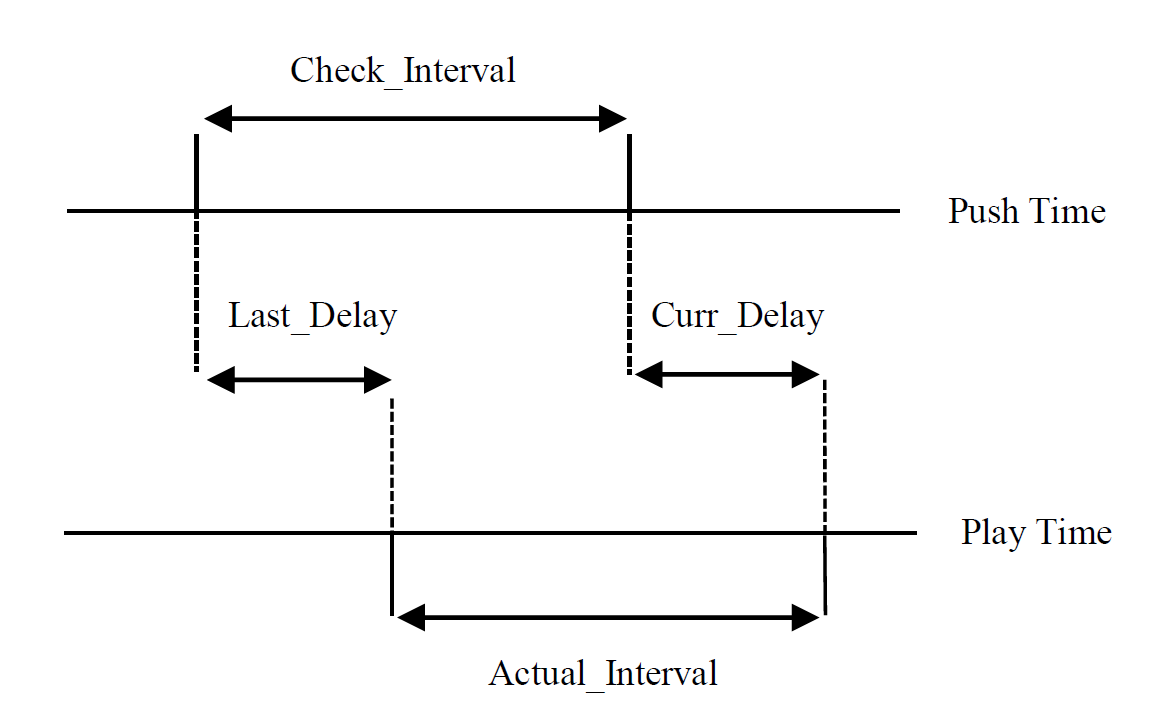
\includegraphics[width = 0.9\linewidth]{figures/Intervals.png}
	\caption{达尔文流媒体服务器中的两个时间线 \label{fig:intervals}}
\end{figure}

在达尔文流媒体服务器中,有两个时间线非常重要。第一个是推送时间线(push time),也就是视频数据包被推送到缓冲区的时间;第二个是播放时间线(play time),也就是数据包应该在播放中被显示的时间(通常记作该数据包的PTS)。这两个时间线的关系如图\ref{fig:intervals}所示。服务器程序会定时检测这两个时间线,并根据数据包的延迟来决定是否需要调整发送的视频质量。图\ref{fig:intervals}中的两个间隔,即检测间隔(check interval)和实际间隔(actual interval),值得我们注意。在理想情况下,每次检测间隔中服务器推送的数据量应该恰好能实际播放等于检测间隔的一段时间,也就是\textit{actual\_interval} = \textit{check\_interval}。如果实际间隔小于检测间隔,说明这段时间内推送了较少的数据,推送数据变慢很可能是带宽有所下降。反过来,如果实际间隔大于检测间隔,说明这段时间内推送了较多的数据,意味着网络条件良好且数据被快速推向客户端。这两个间隔的比值,也就是所谓的“实际与检测间隔比”,能够反映当前推送的速率是否与网络带宽相符。

“实际与检测间隔比”适合用作质量控制有三方面的原因。第一,这个比例直接对应着适合带宽的码率与当前传输的码率的比值,只需据此进行调整就可以准确地使码率符合带宽。第二,根据定义这个比例的理想值就是1,这就是算法的控制目标,无需再通过别的方法确定。第三,这个值在实际系统中便于计算,普适性较好。

\subsection{控制模型}

在通常的PID控制器中,控制输出是用过程变量与控制目标之间的差值进行比例、积分、微分求取出来的。考虑到我们所选的过程变量是一个比例,且控制目标是1,本文对通常的PID控制器做了修改,提出了一个基于比例的模型。在这个模型中,过程变量直接被用来计算控制器输出,而且所有求差的运算都被适当的改为了求比例的运算,以保持模型的合理正确性,如下所示:

\begin{equation}
\label{eq:ut}
{u_t} = {K_p} \cdot E_p^t + {K_i} \cdot E_i^t + {K_d} \cdot E_d^t ,
\end{equation}

\begin{equation}
\label{eq:ep}
E_p^t = \frac{{actual\_interva{l_t}}}{{check\_interva{l_t}}} ,
\end{equation}

\begin{equation}
\label{eq:ei}
E_i^t = \frac{{long\_actual\_interva{l_t}}}{{long\_check\_interva{l_t}}} ,
\end{equation}

\begin{equation}
\label{eq:ed}
E_d^t = E_p^t/E_p^{t - 1} ,
\end{equation}

\begin{equation}
\label{eq:long-actual}
long\_actual\_interva{l_t} = \sum\limits_{\tau = {T_l}}^t {actual\_interva{l_\tau}} ,
\end{equation}

\begin{equation}
\label{eq:long-check}
long\_check\_interva{l_t} = \sum\limits_{\tau = {T_l}}^t {check\_interva{l_\tau}} .
\end{equation}

在公式(\ref{eq:ut})中:$K_p$、$K_i$、$K_d$分别表示比例部分、积分部分、微分部分的可调参数;$E_p^t$、$E_i^t$、$E_d^t$则对应各部分在第t次检测时的值,它们的定义如公式(\ref{eq:ep})至(\ref{eq:long-check})所示;控制器输出$u_t$将用来计算适合当前带宽的码率,并据此选择要传送的质量等级。

在公式(\ref{eq:long-actual})和(\ref{eq:long-check})中,$T_l$代表上一次质量等级改变的时间。按照理论定义,积分部分应该从系统启动开始记录,但在实际环境中,网络带宽有可能变动非常大,如果积分部分记录累积太长时间将不适合反映当前的网络条件,从而减缓调整质量的决策。因此这里采用了一个折衷,选择从上一次质量等级变化的时间开始计算积分部分。

这个基于比例的模型对于所选的过程变量和控制目标比通用模型更加简单有效。而且,在该模型中,当三个参数进行归一化处理后,控制器输出具备明显直观的意义。从公式(\ref{eq:ep})至(\ref{eq:long-check})容易看出,$E_p^t$、$E_i^t$、$E_d^t$这三个值都是在1附近波动的比值;而根据公式(\ref{eq:ut}),控制器输出$u_t$可以被视作这三个比值的加权平均(三个参数作为权值)。因此,$u_t$也是一个在1附近的比值,它对应着适合当前带宽的码率与当前发送码率的关系。换句话说,如果$u_t$大于1,那么控制器决定当前发送码率需要增加;反之,如果$u_t$小于1,意味着控制器认为当前发送码率需要减小。用$u_t$作为一个乘子来调整当前发送的码率,我们就能控制流媒体系统符合带宽的变化。

\subsection{自适应算法}

综上,本文提出的码率自适应算法描述如下:

\begin{algorithm}
	\caption{基于PID的码率自适应算法}
	\label{algo:control}
	\begin{algorithmic}
		\STATE 准备发送数据包
		\STATE check\_interval = curr\_time -- last\_check\_time
		\STATE actual\_interval = curr\_media\_time -- last\_check\_media\_time
		\STATE long\_check\_interval += check\_interval
		\STATE long\_actual\_interval += actual\_interval
		\STATE 根据公式(\ref{eq:ep}) - (\ref{eq:ed})计算$E_p^t$、$E_i^t$、$E_d^t$的值
		\STATE output = ${K_p} \cdot E_p^t + {K_i} \cdot E_i^t + {K_d} \cdot E_d^t$
		\STATE new\_bitrate = output * curr\_bitrate
		\STATE new\_level = get\_level(new\_bitrate, bitrate\_of\_level[])
		\IF {质量等级变化}
		\STATE long\_check\_interval = 0
		\STATE long\_actual\_interval = 0
		\STATE curr\_bitrate = bitrate\_of\_level[new\_level]
		\ENDIF
		\STATE 根据新的质量等级发送数据包
	\end{algorithmic}
\end{algorithm}

相比于其他的调度策略,这个基于PID的自适应算法具有以下几个优点。首先,该算法不仅仅依据当前状态或者固定时间点的信息来做决策,因此质量调整可以在任何合适的时间发生。其次,因为PID模型(微分部分)在某种程度上考虑了对未来的预测,该算法能够判断带宽在未来一段时间内是否会变得足够大或足够小,因此能避免一些不必要的调整。最后,该算法并不一定一次只调整一个质量等级,这就使得当带宽剧烈下降时能够快速下调质量以保证流畅播放,而当系统启动时能够快速上调质量以使用户尽早收到更清晰的视频。

\subsection{参数选取与调优}

与工业界的其他PID控制系统一样,本文提出的算法中三个参数的选取也是跟实现相关的。大多数情况下,为取得最优的效果,需要手动试错调节。每个参数对系统的不同方面产生影响,知道这些影响有助于进行参数选取。一般来说,PID控制器中的比例部分会影响系统的稳定性。如果比例增益$K_p$过高,系统容易变得不稳定。但是,太低的$K_p$又会导致过长的上升时间,使系统响应迟缓。积分部分除了能消除稳态误差,还能加速过程变量向控制目标的变化。这意味着,增大$K_i$能减小上升时间,提高系统的响应速度。但是,积分部分会累积过去一段时间的误差,使过程变量容易超出目标值(即超调),因此过大的$K_i$也会导致系统不稳定。上述这些隐患都能通过微分部分来校正。微分部分通过预测系统行为,具有减小超调、提高稳定性的双重效果。但是微分部分的特点是对误差分成敏感,也正是因为此,工业实践中微分增益$K_d$通常都设置的比较低。

本文采用了经典的Ziegler--Nichols方法\supercite{Ziegler1942}来进行参数选取。该方法首先把积分和微分参数设为0,调节比例参数$K_p$到系统开始震荡时的值$K_u$,假设震荡周期为$T_u$,那么设置$K_p = 0.6K_u$、$K_i = 2K_u/T_u$、$K_d = K_u \cdot T_u/8$。再将$K_p$、$K_i$和$K_d$进行归一化,就得到最终的参数:$K_p = 0.22$,$K_i = 0.73$,$K_d = 0.05$。

\section{实验结果}

\section{本章小结}